\documentclass[withoutpreface,bwprint]{cumcmthesis} %去掉封面与编号页,电子版提交的时候使用。

\usepackage[framemethod=TikZ]{mdframed}
\usepackage{url}   % 网页链接
\usepackage{subcaption} % 子标题
\usepackage{mathtools}

\bibliographystyle{plain}

\title{“FAST”主动反射面的形状调节}
\begin{document}

\maketitle
\begin{abstract}
本文研究我国具有自主知识产权的射电望远镜中国天眼---“FAST”的反射面板从基准态调整到工作态的这一过程,
并分析工作态时馈源舱接收到的有效信号与反射面的反射信号之比。

问题一要求在观测天体发射的电磁波竖直向下的情况下,并考虑反射面板调节因素的,确定理想抛物面。
我们通过数据拟合观测确定具体的基准球面方程。在 $z$ 轴负半轴一定范围内通过蒙特卡洛法枚举抛物面顶点
的坐标,并以口径筛选后剩余主索结点的总调节长度最小为原则,使用变步长法解得抛物面顶点的坐标为
$(0,0,-300.90527)$,从而得到抛物面方程为:$x^2+y^2=562.3456(z+300.9053)$

问题二要求观测天体坐标在 $\alpha =26.795^\circ,\beta =78.169^\circ$的情况下,确定理想抛物面方
程并给出主索结点的调节方案。
通过分析旋转基准球面和旋转抛物面的运算代价,我们最终选择旋转基准球面来固定抛物线开口仍沿 $z$ 轴,
对于旋转之后主索节点坐标的计算,我们选择使用Hamilton四元数\cite{Hamilton2006}和罗德里格旋转公式
推导一个引理,用其结论得到主索节点旋转后的坐标点。
这样理想抛物面的顶点始终在 $z$ 轴的负半轴上且抛物面以 $z$ 轴为对称轴。之后使用问题一的理想抛物面求
解过程,求解旋转后的理想抛物面顶点。再利用旋转的逆运算将顶点旋转回题目所给空间直角坐标系中即可求得
理想抛物面的顶点。同时,根据旋转后坐标系中主索节点工作态的坐标,可计算各个主索节点对应促动器的伸缩量。
根据主索节点的编号以及对应促动器的伸缩量可计算出题目所给坐标系中工作态主索节点的坐标。最终理想抛物面
的顶点坐标为 $(-49.39983133,-36.9490723,-294.4942374)$,完整的结果保存在了附录4.xlsx表格中。

问题三要求基于问题二的反射面调节方案,计算调节后馈源舱的接收比。我们首先需要筛选以出工作区内主索
节点为顶点的反射面板,将筛选结果记入表格work\_triangle-s.xlsx(表格已存入支撑材料)。对于其中一个
反射面板,我们选取三角形反射面板的三个顶点为标准计算法向量,通过反射原理与立体解析几何计算光束经过
工作区域内反射面板到达馈源舱有效区域所在平面的位置,由于反射面板面积远大于有效区域面积,我们计算馈
源舱中心是否在反射后的光束中来确定反射的电磁波是否被接收,经过对工作态300m口径内所有反射面板的计算,
我们得到 $1300$ 个反射面板中 $385$ 个面板反射的光束被有效接收,得到调节后馈源舱接收比:
$p1 = 29.62\%$,同理,我们对于整个基准反射球面的所有主索结点进行计算,得到未经调整的馈源舱接收比:
$p2 = 10.02\%$。经过对比,调整为工作态能将馈源舱的接收比大幅度提高(提高了 $195.6\%$)。

\keywords{Hamilton四元数\quad 罗德里格旋转公式\quad 空间解析几何\quad 蒙特卡洛法\quad
            优化模型}
\end{abstract}

%目录  2019 明确不要目录,我觉得这个规定太好了
%\tableofcontents

%\newpage

\section{问题重述}
中国天眼——$500$米口径球面射电望远镜(Five-hundred-meter Aperture Spherical radio
Telescope,简称 FAST),是我国具有自主知识产权的目前世界上单口径最大、灵敏度最高的
射电望远镜。它的落成启用,对我国在科学前沿实现重大原创突破、加快创新驱动发展具有重
要意义。

FAST 由主动反射面、信号接收系统(馈源舱)以及相关的控制、测量和支承系统组成,其中
主动反射面系统是由主索网、反射面板、下拉索、促动器及支承结构等主要部件构成的一个可
调节球面。主索网由柔性主索按照短程线三角网格方式构成,用于支承反射面板(含背架结
构),每个三角网格上安装一块反射面板,整个索网固定在周边支承结构上。每个主索节点连
接一根下拉索,下拉索下端与固定在地表的促动器连接,实现对主索网的形态控制。反射面板
间有一定缝隙,能够确保反射面板在变位时不会被挤压、拉扯而变形。

主动反射面可分为两个状态:基准态和工作态。基准态时反射面为半径约 $300$ 米、口径为
$500$ 米的球面(基准球面);工作态时反射面的形状被调节为一个 $300$ 米口径的近似旋转抛物
面(工作抛物面)。馈源舱接收平面的中心只能在与基准球面同心的一个球面(焦面)上移动,两同
心球面的半径差为 F=$0.466$R(其中 R 为基准球面半径,称 F/R 为焦径比)。馈源舱接收信号
的有效区域为直径 $1$ 米的中心圆盘。当 FAST 观测某个方向的天体目标时,馈源舱接收平面的中
心被移动到天体目标与基准球面的球心连成的直线与焦面的交点处,调节基准球面上的部分反射面板
形成以天体目标与基准球面的球心连成的直线为对称轴、以馈源舱接收信号为焦点的近似旋转
抛物面,从而将来自目标天体的平行电磁波反射汇聚到馈源舱的有效区域。

将反射面调节为工作抛物面是主动反射面技术的关键,该过程通过下拉索与促动器配合来
完成。下拉索长度固定。促动器沿基准球面径向安装,其底端固定在地面,顶端可沿基准球面
径向伸缩来完成下拉索的调节,从而调节反射面板的位置,最终形成工作抛物面。

本赛题要解决的问题是:在反射面板调节约束下,确定一个理想抛物面,然后通过调节促
动器的径向伸缩量,将反射面调节为工作抛物面,使得该工作抛物面尽量贴近理想抛物面,以
获得天体电磁波经反射面反射后的最佳接收效果。

请你们团队根据附录中的要求及相关参数建立模型解决以下问题:
\begin{enumerate}
    \item 当待观测天体 $𝑆$ 位于基准球面正上方,即 $\alpha = 0°$, $\beta = 90°$ 时,结合考虑反
          射面板调节因素,确定理想抛物面。
    \item 当待观测天体 $𝑆$ 位于 $\alpha = 36.795°$, $\beta = 78.169°$ 时,确定理想抛物面。
          建立反射面板调节模型,调节相关促动器的伸缩量,使反射面尽量贴近该理想抛物面。将理想抛物面
          的顶点坐标,以及调节后反射面 $300$ 米口径内的主索节点编号、位置坐标、各促动器的伸缩量等
          结果按照规定的格式(见附件 $4$)保存在“result.xlsx”文件中。
    \item 基于第 $2$ 问的反射面调节方案,计算调节后馈源舱的接收比,即馈源舱有效区域接收到
          的反射信号与 $300$ 米口径内反射面的反射信号之比,并与基准反射球面的接收比作比较。
\end{enumerate}

\section{问题分析}
\subsection{问题一分析}
在 $\alpha = 0^\circ , \beta = 90^\circ$ 的情况中,天体位于“FAST”射电望远镜的正上方。所以可以使用
本题所给出的三维空间模型进行求解。考虑到反射调节因素,本文期望能尽可能少的移动主索节点来使反射面从球面
变为抛物面。

本文首先在比 $300m$ 口径稍大的范围内筛选一些主索节点。通过遍历抛物面顶点的坐标,再调节各个
主索节点的位置,使它们尽量位于抛物面上。然后以 $300m$ 口径的范围为条件去筛选修正过位置的主索节点。筛选
出符合条件的主索节点后计算所有主索节点移动距离之和。先通过大步长粗略搜索找到较小值的范围,然后通过小步
长来精确搜索得出精确度较高的模型的解。将所有主索节点移动距离之和最小时的抛物面顶点坐标作为理想抛物面顶
点。
\subsection{问题二分析}
在 $\alpha = 36.795^\circ , \beta = 78.169^\circ$ 的情况中,直接使用本题所给出的三维空间难以计算
出抛物面的顶点。本文通过旋转坐标系来建立一个抛物面开口方向与 $z$ 轴正方向相同的空间直角坐标系,以
此简化计算。

由于 $\alpha = 36.795^\circ , \beta = 78.169^\circ$,所以坐标系需要进行两次绕轴旋转。
本文使用Hamilton四元数,将三维空间中的两次旋转等效为一次旋转。再计算出一次旋转的旋转轴和旋转角度,
之后利用罗德里格旋转公式将附件1中的基准球面上主索节点的坐标转换到新的坐标系中。然后利用问题一中的方法
找出抛物面顶点的坐标。再通过逆用之前的旋转公式将求得的抛物面顶点坐标转换为题目所给坐标系中的坐标。最后
利用由两点间距离公式计算出的新坐标系中工作态主索节点坐标与基准球面主索节点坐标间距离来求得各个主索节点
的促动器顶端的径向伸缩量,再通过伸缩量在原坐标系中得到原坐标系工作态主索节点的位置。
\subsection{问题三分析}
题目要求基于第 2 问的反射面调节方案,计算调节后馈源舱的接收比。我们根据调整后主索结点编号与附件3
选出完全位于工作抛物面内的三角形反射面,然后利用反射公式和解析几何,使得来自目标天体的电磁波根据三
角形平面的法线作对称变换,将入射到三角形三个顶点的电磁波分别作对称变换后以平面连接,可以得到三角电
磁波束。

将电磁波束按照方向映射到馈源舱有效区域所在平面得到平面三角形,从而在同一平面上计算电磁波束被馈源
舱接收的量。最终将对于来自天体的平行电磁波的馈源舱接收量与基准球面上有效区域三角形接收量相除,得
到馈源舱有效区域接收到的反射信号与 $300$ 米口径内反射面的反射信号之比。用相同的方法对射向整个基
准球面的电磁波进行变换,计算馈源舱接收量,与基准球面上有效区域三角形接收量相除,得到基准反射球面
的接收比。
\section{模型建立}
\subsection{符号说明及名词解释}
\subsubsection{符号说明}
\begin{center}
    \begin{tabular}{cc}
        \hline
        \makebox[0.3\textwidth][c]{符号} & \makebox[0.4\textwidth][c]{意义}               \\
        \hline
        $\alpha$                         & 方位角 \\
        \hline
        $\beta$                          & 仰角 \\
        \hline
        $R$                              & 基准态时反射面半径(m)                         \\
        \hline
        $C$                              & 基准球面球心 \\
        \hline
        $P$                              & 馈源舱中心  \\
        \hline
        $d$                              & 单个促动器的伸缩量 \\
        \hline
        $p_1$                           & 调节后馈源舱的接收比 \\
        \hline
        $p_2$                           & 基准反射球面的接收比 \\
        \hline
    \end{tabular}
\end{center}
\subsubsection{名词解释}
\begin{enumerate}
    \item 接收比:馈源舱有效区域接收到的反射信号与反射面的反射信号之比。
    \item 旋转矩阵:是在乘以一个向量的时候有改变向量的方向但不改变大小的效果并保持了手性的矩阵。
\end{enumerate}
\subsection{问题一}
\subsubsection{模型的建立}
因为 $\alpha = 0^\circ ,\beta = 90^\circ$ 且题目所给的坐标系以基准球面的球心为原点,
所以本文直接使用题目所给的空间直角坐标系。工作态所需的口径为 $300m$,基准球面半径约为 $300m$,
本文通过附件1中所给出的数据并利用两点间距离公式获得较为精确的半径为 $300.4m$。由于所需的
口径为 $300m$,然而在由基准球面调节为工作态时各主索节点与 $z$ 轴的距离会发生改变,而 $z$ 轴同时
是抛物面的中心对称轴,也是工作态的中轴,所以需要在 $300m$ 口径的范围上增加一定长度 $\xi m$,
在调整主索节点位置之后,再利用准确的 $300m$ 口径去筛选符合条件的主索节点。

\textbf{Step 1:初筛选范围的确定}

工作抛物面顶点处的法线与基准球面口径为 $300m$ 处的边界点和球心的连线成大约 $30^\circ$ 的
角,如图 \ref{fig:range} 中左图所示。在基准状态下,促动器的径向伸缩范围为$-0.6\sim +0.6m$,则在水
平方向上的伸缩范围为 $-0.3\sim +0.3m$(如图 \ref{fig:range} 中右图所示),所以 $\xi = 0.3$。
所以在坐标范围 $x^2 + y^2 \leqslant (150 + \xi)^2$ 中,筛选出应当调节的主索节点。
\begin{figure}[!h]
    \centering
    \begin{minipage}[c]{0.48\textwidth}
        \centering
        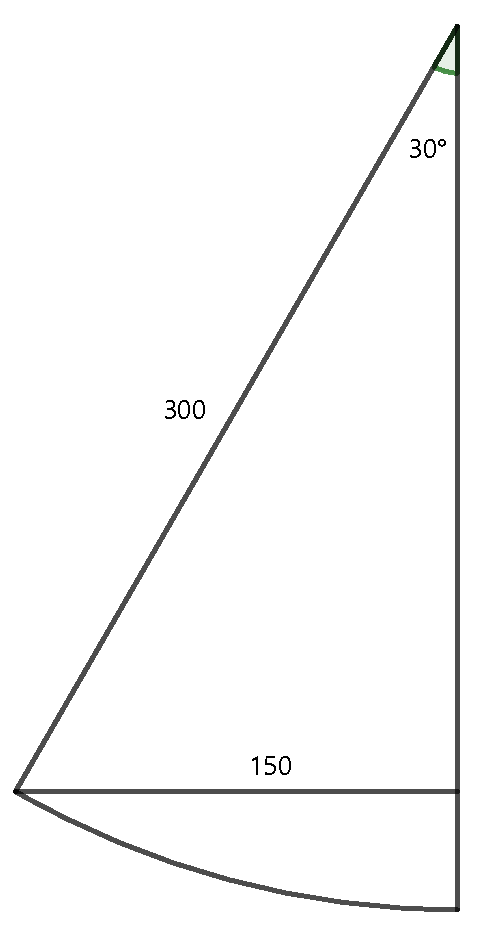
\includegraphics[height=0.2\textheight]{angle1.pdf}
    \end{minipage}
    \begin{minipage}[c]{0.48\textwidth}
        \centering
        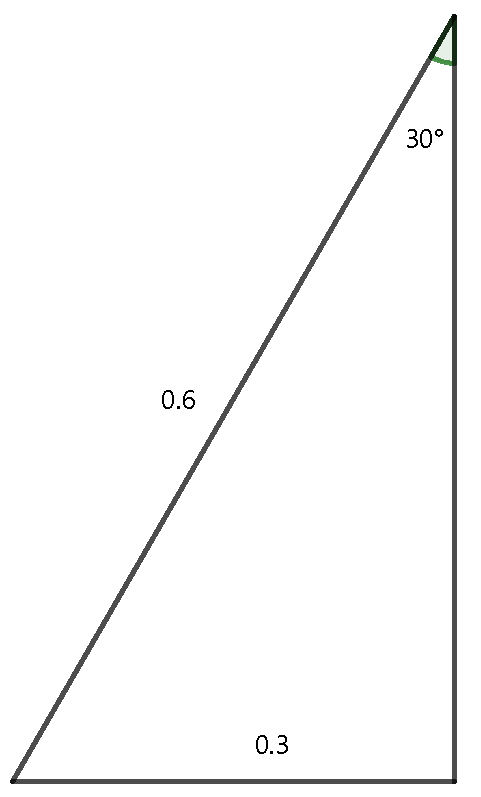
\includegraphics[height=0.2\textheight]{angle2.pdf}
    \end{minipage}
    \caption{}
    \label{fig:range}
\end{figure}

\textbf{Step 2:抛物面顶点打靶范围的确定}

对于理想抛物面顶点的位置,本文采用蒙特卡洛法,对抛物面顶点进行打靶,搜索使由基准球面到工作态所有
筛选出的主索节点移动距离之和最小的抛物面顶点位置。

对于打靶范围的选择,由于促动器顶端径向伸缩量的范围是 $-0.6\sim +0.6m$。当抛物面顶点位置距离基准
球面过远时,绝大多数促动器所需调节的距离可能超过 $-0.6\sim +0.6m$。随着顶点由基准球面圆心向下移
动,调节距离之和呈现先减小后增大的趋势。在贴近基准球面处其值较小,故本文选择的范围为$\left[R-1.2,
R+1.2\right]m$。

\textbf{Step 3:理想工作态主索节点坐标的求解}

若抛物面的顶点为 $(0,0,-a)$,可以通过焦点 $P$ 和顶点,进而确定抛物面的方程,记 $p$ 为焦距,
$p = a-R \times 0.534$,抛物面的公式为
\begin{equation}
    \label{eq:paraboloid}
    x^2 + y^2 = 4p(z + a)
\end{equation}

由于促动器伸缩沿基准球面径向,所以主索节点的位置移动均在一条过基准球面球心的直线上,可以通过球心
坐标 $(x_c,y_c,z_c)$ 和主索节点坐标 $(x_1,y_1,z_1)$ 计算得这个直线的方程为
\begin{equation}
    \label{eq:line}
    \frac{\displaystyle x - x_c}{\displaystyle x_1 - x_c} = \frac{\displaystyle y - y_c}
    {\displaystyle y_1 - y_c} = \frac{\displaystyle z - z_c}{\displaystyle z_1 - z_c}
\end{equation}

联立方程 \eqref{eq:paraboloid} 与 \eqref{eq:line} 解得忽视促动器调节因素的情况下最理想的主索
节点坐标为
\[
\begin{dcases}
    \smallskip
    x_2 = \frac{(2\times x_1\times (p\times z_1 + \sqrt{p\times (a\times x_1^2 + a\times
    y_1^2 + p\times z_1^2)}))}{(x_1^2 + y_1^2)}  \\
    \smallskip
    y_2 = \frac{(2\times x_1\times (p\times z_1 + \sqrt{p\times (a\times x_1^2 + a\times
    y_1^2 + p\times z_1^2)}))}{(x_1^2 + y_1^2)(x_1 \times y_1)}  \\
    z_2 = \frac{(2\times x_1\times (p\times z_1 + \sqrt{p\times (a\times x_1^2 + a\times
    y_1^2 + p\times z_1^2)}))}{(x_1^2 + y_1^2)(x_1 \times z_1)}  \\
\end{dcases}
\]

\textbf{Step 4:二次筛选}

在调节主索节点的位置后,其中的一些主索节点可能已经超出了口径为 $300m$ 的区域,此时我们对主索节
点再进行一次筛选,将那些超出工作抛物面范围的主索节点去除。选取坐标满足 $x_1 + y_1 \leqslant  150^2$
的主索节点来进行下一步计算。

\textbf{Step 5:求促动器伸缩量}

由主索节点前后位置计算对应促动器的伸缩量d,
\[
    |d| = \sqrt{(x_2-x_1)^2 + (y_2-y_1)^2 + (z_2-z_1)^2}
\]
将移动距离大于 $0.6m$ 的主索节点限制为 $0.6m$,并对所有伸缩量的绝对值求和。在蒙特卡洛法打靶过
程中最终根据总伸缩量最小选取理想抛物面。

\medskip
\textbf{目标:$\min\sum |d|$}
\subsubsection{模型的解}
利用蒙特卡洛法对抛物线顶点进行打靶,先由大步长 $0.1m$ 可将抛物线顶点的数据范围确定在 $300.8m$
到 $301.0m$ 之间,再使用小步长 $0.00001m$ 在 $300.8m \sim 301.0m$ 的范围内进行搜索。\\
%\begin{figure}[!h]
    {\centering
    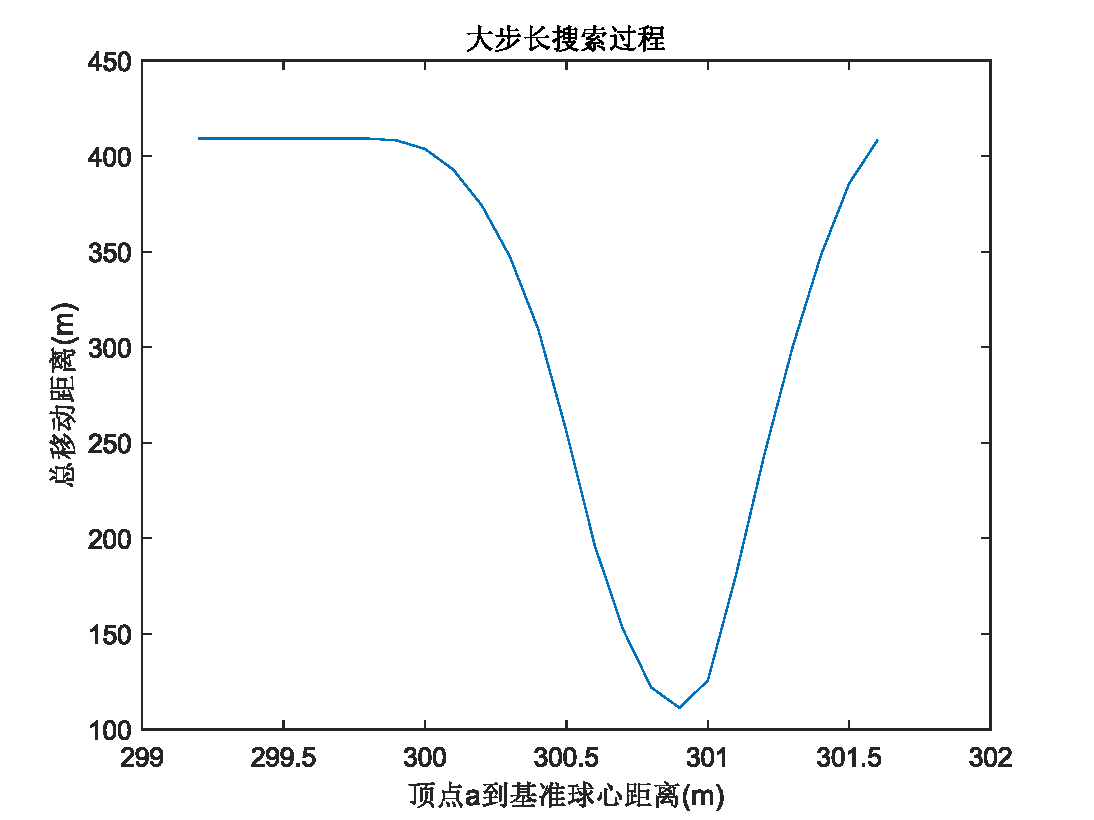
\includegraphics[scale=0.8]{大步长搜索过程.pdf}}
%\end{figure}
\\
%\begin{figure}[!h]
    {\centering
    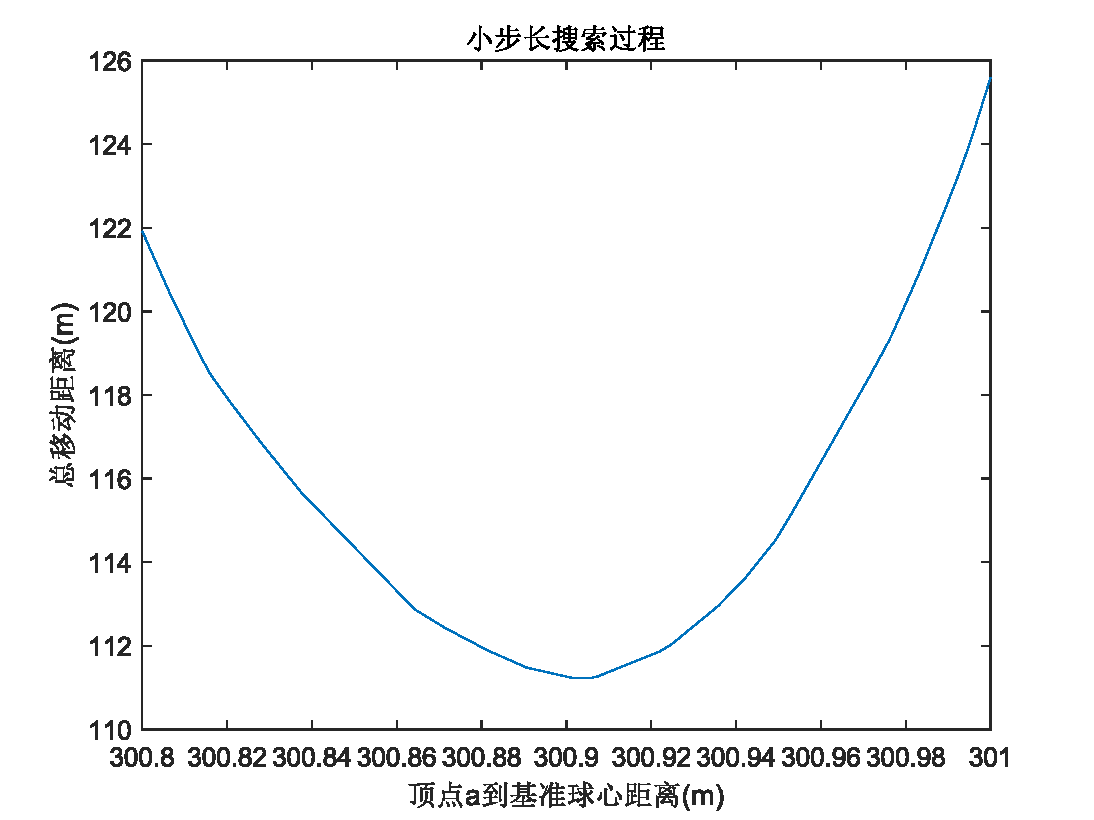
\includegraphics[scale=0.8]{小步长搜索过程.pdf}}
%\end{figure}
\\

最终搜索得出最优值 $a = 300.9053$。可算出 $p = 140.5864$,所以得到的理想抛物面的方程为
\[
    x^2 + y^2 = 562.3456(z + 300.9053)
\]
\subsection{问题二}
\subsubsection{罗德里格旋转公式}
罗德里格旋转公式是在一个三维空间里,以单位向量 $\overrightarrow{n}$ 为旋转轴,在右手方向下旋转角度
为 $\theta$ 时,原空间一个三维空间向量 $\overrightarrow{v}$ 经旋转后可由 $\overrightarrow{v_{rot}}$
表示
\[
    \overrightarrow{v_{rot}} = \overrightarrow{v}\cos\theta + (\overrightarrow{n}
    \times \overrightarrow{v})\sin\theta + \overrightarrow{n}(\overrightarrow{n}
    \times \overrightarrow{v})(1 - \cos\theta) 
\]
\subsubsection{模型的建立}
由于问题 $2$ 天体角度的变化,导致抛物面的开口方向不再沿 $z$ 轴正方向,又由于抛物面绕轴旋转之后
公式过于复杂,本文采用逆向旋转整个基准球面的方法来使抛物面开口始终沿 $z$ 轴正方向。

\textbf{Step 1:旋转方式的分析}

如果旋转抛物面,需要先绕 $z$ 轴(方向向量 $(0,0,1)$)沿右手方向旋转 $\alpha$ 角,此时的旋转矩
阵设为 $R$,再绕 $y$ 轴旋转后的方向向量 $(0,1,0)\cdot R$ 沿右手方向旋转 $90^\circ-\beta$
角。

所以逆向旋转基准球面的方法应为先绕 $(0,1,0)\cdot R$ 沿右手方向旋转 $\beta-90^\circ$ 角,
再绕方向向量 $(0,0,1)$ 沿右手方向旋转 $-\alpha$ 角。其中旋转矩阵 $R$ 为
\[
    \begin{bmatrix}
        \cos(-\alpha) & -\sin(-\alpha) & 0 \\
        \sin(-\alpha) & \cos(-\alpha)  & 0 \\
        0  &  0  & 1 \\
    \end{bmatrix}
\]

\textbf{Step 2:证明旋转叠加的引理1}

对于两次旋转的叠加,本文使用Hamilton四元数和罗德里格旋转公式相结合的方法,证明引理1:
\begin{quote}
    第一次绕 $\overrightarrow{n_1}$ 旋转 $\theta _1$ 角,第二次绕 $\overrightarrow{n_2}$
    旋转 $\theta _2$ 角,那么相当于绕 $\overrightarrow{n}$ 旋转 $\theta$ 角。
    \[
        \begin{split}
            &\cos(\frac{\theta}{2}) = \cos(\frac{\theta _1}{2})
            \cos(\frac{\theta _2}{2}) - (\overrightarrow{n_1} \cdot 
            \overrightarrow{n_2})\sin(\frac{\theta _1}{2})
            \sin(\frac{\theta _2}{2}) \\
            &\overrightarrow{n} = \frac{\displaystyle \overrightarrow{n_1}
            \cos(\frac{\theta _2}{2})\sin(\frac{\theta _1}{2}) + 
            \overrightarrow{n_2}\cos(\frac{\theta _1}{2})
            \sin(\frac{\theta _2}{2}) + \overrightarrow{n_1} \times 
            \overrightarrow{n_2}\sin(\frac{\theta _1}{2})
            \sin(\frac{\theta _2}{2})}
            {\displaystyle \sin(\frac{\theta}{2})} 
        \end{split}
    \]
\end{quote}

\noindent\textbf{证明:}

Hamilton四元数为高阶复数,形如:$q=a+bi+cj+dk$ \par
$i,j,k$ 为虚数,$i^2=j^2=k^2=-1;$
$i \times j=k,$
$i \times k=-j,$
$j \times k=i,$
$j \times i=-k,$
$k \times i=j,$
$k \times j=-i;$ \par
$q=a+bi+cj+dk$ 的共轭四元数为:$q^*=a-bi-cj-dk$ \par
满足:\par
$qq^*=a^2-(bi+cj+dk)^2=a^2+b^2+c^2+d^2-bck+bck-cdi+cdi-bdj+bdj$ \par
\quad\ \ \,$=a^2+b^2+c^2+d^2=|q|^2$ \par
$|q|$ 为 $q$ 的模长。\par
定义 $q$ 的逆为 $q^{-1}=\frac{\displaystyle q^*}{\displaystyle |q|^2}$ \par
可以推出 $q^{-1}q=1$ \par
下面我们先证明:空间中的任意向量 $( x ,y ,z )$,在绕单位向量 $(n_x,n_y,n_z)$旋转 $\theta $
角后(右手方向为正方向),其新的坐标位置由四元数 $r$ 的 $i , j , k$ 分量给出:\par
$r=qpq^{-1},p=xi+yj+zk,$ \par
$q = \cos(\frac{\theta }{2}) + \sin(\frac{\theta }{2})(n_xi + 
    n_yj + n_zk)$ \par
由于 $q$ 的模长为 $1$, 可知 $q^{-1}=q^*$ \par
(为便于计算我们直接将向量的基视为复数) \par
$r = qpq^{-1} = (\cos(\frac{\theta}{2}) + 
\sin(\frac{\theta}{2})\overrightarrow{n})\overrightarrow{p} 
(\cos(\frac{\theta}{2}) - \sin(\frac{\theta}{2})
\overrightarrow{n})$ \par
其中 $pq^{-1} = \overrightarrow{p} (\cos(\frac{\theta}{2}) - 
\sin(\frac{\theta}{2})\overrightarrow{n}) = 
\sin(\frac{\theta}{2})\overrightarrow{n} \cdot \overrightarrow{p} -
\sin(\frac{\theta}{2})\overrightarrow{p} \times \overrightarrow{n} +
\overrightarrow{p} \cos(\frac{\theta}{2})$
\[
    %\begin{array}{l}
    \begin{split}
        r &= qpq^{-1} \\ &= (\cos(\frac{\theta}{2}) - 
        \sin(\frac{\theta}{2})\overrightarrow{n})
        (\sin(\frac{\theta}{2})\overrightarrow{n} \cdot \overrightarrow{p} -
        \sin(\frac{\theta}{2})\overrightarrow{p} \times \overrightarrow{n} +
        \overrightarrow{p}\cos(\frac{\theta}{2})) \\ &= \sin(\frac{\theta}{2})
        \cos(\frac{\theta}{2})\overrightarrow{n} \cdot \overrightarrow{p} -
        (\sin(\frac{\theta}{2})\overrightarrow{n}) \cdot
        [-\sin(\frac{\theta}{2})\overrightarrow{p} \times \overrightarrow{n} +
        \overrightarrow{p}\cos(\frac{\theta}{2})] \\ &\quad + 
        [\sin(\frac{\theta}{2})\overrightarrow{n} \times 
        (-\sin(\frac{\theta}{2})\overrightarrow{p} \times \overrightarrow{n} +
        \cos(\frac{\theta}{2})\overrightarrow{p})] + \sin ^2
        (\frac{\theta}{2})(\overrightarrow{n} \cdot \overrightarrow{p})
        \overrightarrow{n} \\ &\quad + \cos ^2(\frac{\theta}{2})\overrightarrow{p} -
        \cos(\frac{\theta}{2})\sin(\frac{\theta}{2})\overrightarrow{p} \times 
        \overrightarrow{n} \\ &= -\sin^2(\frac{\theta}{2})\overrightarrow{n} \times
        (\overrightarrow{p} \times \overrightarrow{n}) +
        \sin^2(\overrightarrow{n} \cdot \overrightarrow{p})\overrightarrow{n} +
        \cos^2(\frac{\theta}{2})\overrightarrow{p} \\ &\quad - 2\cos(\frac{\theta}{2})
        \sin(\frac{\theta}{2})\overrightarrow{p} \times \overrightarrow{n} 
    \end{split}
    %\end{array}
\]
\phantom{哈哈}代入,得:\par
原式 $= \cos(\theta)\overrightarrow{p} - \sin(\theta)\overrightarrow{p} \times
\overrightarrow{n} + 2\sin^2(\frac{\theta}{2})(\overrightarrow{n} \cdot 
\overrightarrow{p})\overrightarrow{n} = \cos(\theta)\overrightarrow{p} -
\sin(\theta)\overrightarrow{p} \times \overrightarrow{n} +
(1 - \cos(\theta ))(\overrightarrow{n} \cdot \overrightarrow{p})
\overrightarrow{n} $
形式与罗德里格旋转公式相同,所以得证。 \par
我们再证明引理 \par
我们知道两次旋转之后的坐标为 $pqrp^{-1}q^{-1}$ \par
我们记第一次旋转绕向量 $n_1$ 旋转了 $\theta _1$ 角,第二次旋转绕向量 $n_2$ 旋转了 $\theta _2$角,
则第一次旋转得到的坐标为 $prp^{-1}$,第二次旋转得到的坐标为 $qprp^{-1}q^{-1}$,其中
\[
    \begin{split}
        p = \cos(\frac{\theta _1}{2}) + \sin(\frac{\theta _1}{2})n_{1x}i +
        \sin(\frac{\theta _1}{2})n_{1y}j + \sin(\frac{\theta _1}{2})n_{1z}k, \\
        q = \cos(\frac{\theta _2}{2}) + \sin(\frac{\theta _2}{2})n_{2x}i +
        \sin(\frac{\theta _2}{2})n_{2y}j + \sin(\frac{\theta _2}{2})n_{2z}k
    \end{split}
\]

易知,$qp$ 和 $p^{-1}q^{-1}$ 共轭,要证明:
\[
    qp = \cos(\theta) + \sin(\theta)n_xi + \sin(\theta)n_yj +
    \sin(\theta)n_zk
\]

其中 $\theta$ 和 $\overrightarrow{n}$ 待定。
\[
    \begin{split}
        qp &= (\cos(\frac{\theta _2}{2}) + \sin(\frac{\theta _2}{2})n_{2x}i
        + \sin(\frac{\theta _2}{2})n_{2y}j + \sin(\frac{\theta _2}{2})n_{2z}k)
        (\cos(\frac{\theta _1}{2}) + \sin(\frac{\theta _1}{2})n_{1x}i \\ &\quad +
        \sin(\frac{\theta _1}{2})n_{1y}j + \sin(\frac{\theta _1}{2})n_{1z}k) \\
        &= \cos(\frac{\theta _1}{2})\cos(\frac{\theta _2}{2}) - 
        \sin(\frac{\theta _1}{2})\sin(\frac{\theta _2}{2})\overrightarrow{n_1} 
        \cdot \overrightarrow{n_2} + \cos(\frac{\theta _2}{2})
        \sin(\frac{\theta _1}{2})\overrightarrow{n_1} \\&\quad + 
        \cos(\frac{\theta _1}{2})\sin(\frac{\theta _2}{2})\overrightarrow{n_2} +
        \sin(\frac{\theta _1}{2})\sin(\frac{\theta _2}{2})(\overrightarrow{n_1}
        \times n_2)
    \end{split}
\]

我们证明,上式的模为 $1$ \par
实部的平方为:
\begin{align*}
    \cos ^2(\frac{\theta _1}{2})\cos ^2&(\frac{\theta _2}{2}) +
    \sin ^2(\frac{\theta _1}{2})\sin ^2(\frac{\theta _2}{2})
    (\overrightarrow{n_1} \cdot \overrightarrow{n_2})^2 \\ &-
    2\cos(\frac{\theta _1}{2})\cos(\frac{\theta _2}{2})
    \sin(\frac{\theta _1}{2})\sin(\frac{\theta _2}{2})
    \overrightarrow{n_1} \cdot \overrightarrow{n_2} 
\end{align*}

虚部的平方为:
\begin{align*}
    \cos ^2(\frac{\theta _2}{2})&\sin ^2(\frac{\theta _1}{2}) +
    \cos ^2(\frac{\theta _1}{2})\sin ^2(\frac{\theta _2}{2}) \\ & +
    \sin ^2(\frac{\theta _1}{2})\sin ^2(\frac{\theta _2}{2})
    (\overrightarrow{n_1} \times \overrightarrow{n_2})^2 \\ &\quad +
    2\cos(\frac{\theta _1}{2})\cos(\frac{\theta _2}{2})
    \sin(\frac{\theta _1}{2})\sin(\frac{\theta _2}{2})
    \overrightarrow{n_1} \cdot \overrightarrow{n_2} 
\end{align*}

由于 $(\overrightarrow{n_1} \times \overrightarrow{n_2})^2 + (\overrightarrow{n_1} 
\cdot \overrightarrow{n_1})^2 = 1$,易知,实部和虚部平方之和为 $1$。

由此可得:旋转角为
\[
    \begin{split}
        &\cos(\frac{\theta}{2}) = \cos(\frac{\theta _1}{2})
        \cos(\frac{\theta _2}{2}) - (\overrightarrow{n_1} \cdot 
        \overrightarrow{n_2})\sin(\frac{\theta _1}{2})
        \sin(\frac{\theta _2}{2}) \\
        &\overrightarrow{n} = \frac{\displaystyle \overrightarrow{n_1}
        \cos(\frac{\theta _2}{2})\sin(\frac{\theta _1}{2}) + 
        \overrightarrow{n_2}\cos(\frac{\theta _1}{2})
        \sin(\frac{\theta _2}{2}) + \overrightarrow{n_1} \times 
        \overrightarrow{n_2}\sin(\frac{\theta _1}{2})
        \sin(\frac{\theta _2}{2})}
        {\displaystyle \sin(\frac{\theta}{2})} 
    \end{split}
\]\par
\textbf{引理1证毕 $\Box$}

\medskip
\medskip
\medskip
\textbf{Step 3:利用引理以及罗德里格旋转公式计算旋转后的球面}

我们将题目附件 $1$ 中数据引入,使用上文中证明的旋转公式,将基准球面各个点的坐标旋转到新的坐标
系中,使得新坐标系中的抛物面以 $z$ 轴为中轴,且开口沿 $z$ 轴正半轴,并将各点坐标保存到“旋转球
面.xls”文件中。

\textbf{Step 4:利用问题一所得程序求问题二的理想抛物面顶点}
由于抛物面开口仍沿 $z$ 轴正方向,所以可以直接利用问题一所得程序和旋转后的主索节点坐标计算旋转后
的理想抛物面顶点以及各主索节点对应促动器的伸缩量。

由于问题一中仅使用了促动器伸缩量的绝对值,我们需要根据主索节点调节前后的坐标变化,分析伸缩量的正
负。具体过程如下:

根据主索结点调整前后坐标的 $z$ 轴坐标高低,可以判断促动器伸缩量的正负:在旋转后的坐标系中,天体
电磁波的方向是竖直向下,主索节点在 $z$ 轴上的坐标均为负数。所以当促动器伸长时,主索节点更接近球
心,$z$ 轴的坐标将增大。反之,$z$ 轴的坐标将减小。

所以根据
\[
    d = 
    \left\{
        \begin{array}{rl}
            |d|,&z_2>z_1 \\
            -|d|,&z_2<z_1
        \end{array}
    \right.
\]
来判断实际的促动器伸缩量。

\textbf{Step 5:通过旋转的逆运用求解原坐标系中抛物线顶点坐标}

将旋转之后的理想抛物面顶点坐标,再通过引理1的结论:旋转轴不变,旋转角度为 $-\theta$,即可得到题干
所给坐标系中理想抛物面的顶点坐标

\textbf{Step 6:根据伸缩量计算原坐标系中主索节点的位置}

利用上述步骤所计算出的工作态 $300m$ 口径内主索节点的对应编号以及其伸缩量,再根据“附件1.xlsx”中
原坐标系主索节点基准态坐标来计算其工作态的新坐标。
设主索结点在基准球面上的原始坐标为 $(x0, y0, z0)$, 该节点对应促动器的伸缩量为 $d$,
主索结点对应抛物面上的新点坐标为 $(x, y,z)$,计算公式如下:
\[
    \begin{dcases}
        \smallskip
        x = x_0 - \frac{(d*x_0)}{\sqrt{x_0^2+y_0^2+z_0^2}}; \\
        \smallskip
        y = y_0 - \frac{(d*y_0)}{\sqrt{x_0^2+y_0^2+z_0^2}}; \\
        z = z_0 - \frac{(d*z_0)}{\sqrt{x_0^2+y_0^2+z_0^2}};
    \end{dcases}
\]
\subsubsection{模型的解}
首先通过引理1将“附件1.xlsx”中的数据转换为旋转后的坐标数据保存到“旋转球面.xls”。然后利用旋转后的
数据,使用步骤1的理想抛物面求解过程搜索出理想抛物面的坐标,此坐标系中坐标为 $(0,0,-300.88608)$,
同时判断伸缩量的正负,保存到“result.xlsx”中。通过引理1的逆旋转,将顶点坐标转换到原坐标系中,其值
为 $(-49.3998,-36.9491,-294.4942)$。然后根据伸缩量和“附件1.xlsx”中的基准球面坐标计算工作态时
主索节点的坐标,数据存入“result.xlsx”。
\begin{figure}[!h]
    \centering
    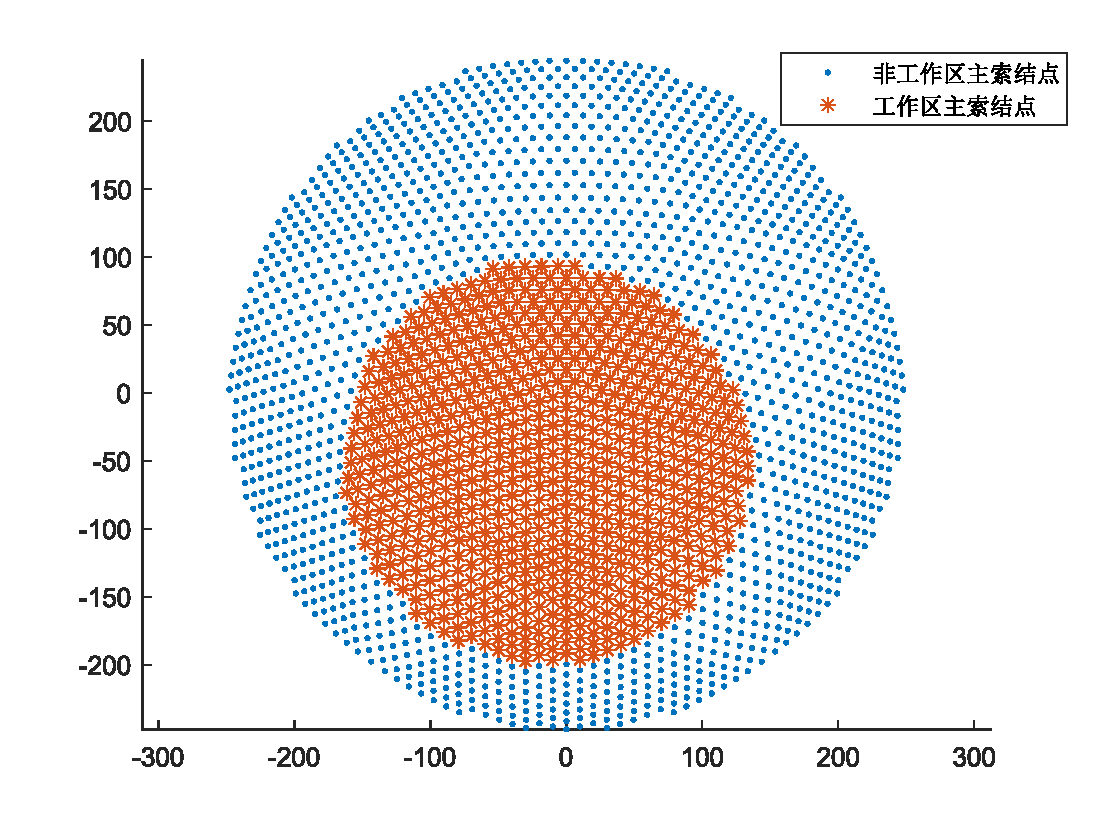
\includegraphics[scale=0.8]{A2.pdf}
    \caption{工作区主索节点示意图}
\end{figure}
\subsection{问题三}
\subsubsection{模型的建立}
由题目数据,馈源舱接收信号的有效区域圆盘面积为 $\frac{\pi}{4} $ 平方米,而估算的三角形反射
面板的面积大约为 $58$ 平方米,反射面板的面积约为馈源舱有效区域的 $73.85$ 倍,由于大小差距巨
大,我们计算馈源舱是否接收到反射面板的信号,可以近似视为判断馈源舱中心是否落在了三角形反射
面板反射的三棱柱形电磁波束中。

\textbf{Step 1:反射电磁波的求解}

我们计算天体平行电磁波经过反射面板后的反射电磁波,首先通过天体的位置 $\alpha = 36.795^\circ,
\beta = 78.169^\circ$,可以得到天体电磁波的方向向量 $\overrightarrow{c} 
(-\cos(\alpha),-\sin(\alpha),-\tan(\beta))$三角形反射面板的顶点坐标可近似为顶点对应的主索
节点的坐标,设顶点坐标为 $(x_0,y_0,$\\$z_0)$,通过顶点坐标和电磁波的方向向量,我们可以得到射向这
个顶点的电磁波的直线方程:
\[
    \frac{x-x_0}{-\cos\alpha} = \frac{y-y_0}{-\sin\alpha} = \frac{z-z_0}{-\tan\beta} 
\]

利用三角形三个顶点的坐标,可以计算出三角形的法向量,记为 $\overrightarrow{n}=(n_1,n_2,n_3)$。
同样可以利用三角形的顶点和 $\overrightarrow{n} $ 计算出顶点处电磁波反射的法线,利用法线和入
射光线可以计算出射光线,具体过程如下:

取入射直线上区别于三角形顶点的一个点,本文统一采用三角形顶点的 $z$ 轴坐标 $+10$ 的点,
此点坐标暂记为点 $T(x_t,y_t,z_t)$,其中
\[
    \begin{dcases}
        x_t=x_0+\frac{10\cos(\alpha)}{\tan(\beta)} \\
        y_t=y_0+\frac{10\sin(\alpha)}{\tan(\beta)} \\
        z_t=z_0+10
    \end{dcases}
\]

计算法线和入射直线的夹角:$\cos(\theta)=\frac{\displaystyle\overrightarrow{n}\overrightarrow{c}}
{\displaystyle|n||c|}$

\smallskip
$T$ 与顶点的距离:$\delta=\displaystyle\sqrt{10^2+(\frac{\displaystyle10\cos(\alpha)}
{\displaystyle\tan(\beta)})^2+(\frac{\displaystyle10\sin(\alpha)}{\displaystyle\tan(\beta)})^2}$

$T$ 点到法线的垂足记为 $R(x_r,y_r,z_r)$

$R$ 到顶点的距离为 $D=\delta\cdot \cos(\theta)$

可以得到
\[
    \begin{dcases}
        x_r=x_0+n_1 \cdot\frac{d}{\sqrt{n_1^2+n_2^2+n_3^2}}  \\
        y_r=y_0+n_2 \cdot\frac{d}{\sqrt{n_1^2+n_2^2+n_3^2}}  \\
        z_r=z_0+n_3 \cdot\frac{d}{\sqrt{n_1^2+n_2^2+n_3^2}}  \\
    \end{dcases}
\]


设 $T$ 关于法线的对称点为 $T'(x_{tt},y_{tt},z_{tt})$

通过向量 $\overrightarrow{TT'}=2\overrightarrow{TR}$

可以计算出:
\[
    \begin{dcases}
        x_{tt}=2x_r-x_t \\
        y_{tt}=2y_r-y_t \\
        z_{tt}=2z_r-z_t \\
    \end{dcases}
\]

得到反射直线:
\[
    \frac{x-x_0}{2x_R-x_t-x_0} = \frac{y-y_0}{2y_R-y_t-y_0} = 
    \frac{z-z_0}{z_R-z_t-z_0}
\]

\textbf{Step 2:求反射电磁波与有效区域平面的交点}

馈源舱中心的坐标 $P(x_p,y_p,z_p)$ 可以利用
\[
    \begin{dcases}
        -\frac{x_p}{\cos\alpha} = -\frac{y_p}{\sin\alpha} = -\frac{z_p}{\tan\beta} \\
        x_p^2 + y_p^2 + z_p^2 = (R \cdot 0.534)^2
    \end{dcases}
\]
求出 $P(-\cos\alpha\cdot t_0,-\sin\alpha \cdot t_0,-\tan\beta\cdot t_0)$,其中
$t_0 = 0.534R\cos\beta$

选取馈源舱有效区域圆盘所在的平面,平面的表达式可以用点法式写出:
\[
    -\cos\alpha(x + t_0\cos\alpha) - \sin\alpha(y + t_0\sin\alpha) - 
    \tan\beta(z + t_0\tan\beta) = 0 
\]

将反射直线与平面的表达式联立:
\[
    \begin{dcases}
        \frac{x-x_0}{2x_R-x_t-x_0} = \frac{y-y_0}{2y_R-y_t-y_0} = 
        \frac{z-z_0}{z_R-z_t-z_0}  \\
        -\cos\alpha(x + t_0\cos\alpha) - \sin\alpha(y + t_0\sin\alpha) - 
        \tan\beta(z + t_0\tan\beta) = 0 
    \end{dcases}
\]
可以解出反射到有效区域平面的点的坐标

\textbf{Step 3:判断馈源舱是否在接收到反射电磁波中}

由于第二步求得与中心共面的三个点,判断馈源舱中心是否接收到反射电磁波可以视为判断,馈源舱中心是否
在反射所得的三个点围成的三角形内,判断方法可以利用几何性质:三角形内一点到三顶点的向量两两夹角之
和为 $360^\circ$,而三角形外一点到三顶点的向量两两夹角之和小于 $360^\circ$。
\subsubsection{模型的解}
分别引入问题 $2$ 所得数据“附件4.xlsx”,和基准球面数据“附件1.xlsx”以及“附件3.xlsx”,首先利用“附
件4.xlsx”中的工作口径内主索节点的编号,在“附件3.xlsx”中筛选所有以工作口径内主索节点为三顶点的反
射面板,将筛选结果输出为“work\_triangles.xlsx”保存在支撑材料中。

对于每个在“work\_triangles.xlsx”中的三角形面板,可利用模型和“附件4.xlsx”中的数据解出其反射电
磁波是否被接收,对于所有“附件3.xlsx”中的反射面板,可利用模型和“附件1.xlsx”中的数据解出基准球面
时的反射面板反射电磁波是否会被接收。

最终计算结果为:基于第 $2$ 问的反射面调节方案,调节后馈源舱的接收比为 $p1 = 29.62\%$。对于整个基
准反射球面计算,得到未经调整的馈源舱接收比:$p2 = 10.02\%$。
\bibliography{references}
\begin{appendices}
\section{第一问MATLAB代码一(大步长)}
\begin{lstlisting}[language=matlab]
clear all, clc;

%读入数据
data = xlsread("附件1.csv", 1, 'B2:D2227');%(n*3的矩阵)
data2 = [];
cnt2 = 0;
for i = 1:2226
    x = data(i,1);
    y = data(i,2);
    z = data(i,3);
    if x^2+y^2 <= 150.3^2
        data2 = [data2; i, x, y, z];
        cnt2 = cnt2 + 1;
    end
end
anss = inf;
finala = 0;
for a = 300.4-1.2:0.1:300.4+1.2
    s = 0;
    p = a-300.4*0.534;
    for i = 1:cnt2
        num = data2(i,1);
        x2 = data2(i,2);
        y2 = data2(i,3);
        z2 = data2(i,4);
        ansx1 = (2*x2*(p*z2 + sqrt(p*(a*x2^2 + a*y2^2 + p*z2^2))))/(x2^2 + y2^2); 
        ansy1 = ansx1 / x2 * y2;
        ansz1 = ansx1 / x2 * z2;
        ansx2 = (2*x2*(p*z2 - sqrt(p*(a*x2^2 + a*y2^2 + p*z2^2))))/(x2^2 + y2^2);
        ansy2 = ansx2 / x2 * y2;
        ansz2 = ansx2 / x2 * z2;
        if ansz2 < ansz1
            ansx = ansx2;
            ansy = ansy2;
            ansz = ansz2;
        else
            ansx = ansx1;
            ansy = ansy1;
            ansz = ansz1;
        end
        if ansx^2 + ansy^2 <= 150^2
            s = s + sqrt((ansx - x2)^2 + (ansy - y2)^2 + (ansz - z2)^2);
        end
    end
    if anss > s
        anss = s;
        finala = a;
    end
end
finala

\end{lstlisting}
\section{第一问MATLAB代码二(小步长)}
\begin{lstlisting}[language=matlab]
clear all, clc;

%读入数据
data = xlsread("附件1.csv", 1, 'B2:D2227');%(n*3的矩阵)
data2 = [];
cnt2 = 0;
for i = 1:2226
    x = data(i,1);
    y = data(i,2);
    z = data(i,3);
    if x^2+y^2 <= 150.3^2
        data2 = [data2; i, x, y, z];
        cnt2 = cnt2 + 1;
    end
end
anss = inf;
finala = 0;
for a = 299:0.00001:301
    s = 0;
    p = a-300.4*0.534;
    for i = 1:cnt2
        num = data2(i,1);
        x2 = data2(i,2);
        y2 = data2(i,3);
        z2 = data2(i,4);
        ansx1 = (2*x2*(p*z2 + sqrt(p*(a*x2^2 + a*y2^2 + p*z2^2))))/(x2^2 + y2^2); 
        ansy1 = ansx1 / x2 * y2;
        ansz1 = ansx1 / x2 * z2;
        ansx2 = (2*x2*(p*z2 - sqrt(p*(a*x2^2 + a*y2^2 + p*z2^2))))/(x2^2 + y2^2);
        ansy2 = ansx2 / x2 * y2;
        ansz2 = ansx2 / x2 * z2;
        if ansz2 < ansz1
            ansx = ansx2;
            ansy = ansy2;
            ansz = ansz2;
        else
            ansx = ansx1;
            ansy = ansy1;
            ansz = ansz1;
        end
        if ansx^2 + ansy^2 <= 150^2
            tmps = sqrt((ansx - x2)^2 + (ansy - y2)^2 + (ansz - z2)^2);
            if tmps > 0.6
                tmps = 0.6;
            end
            s = s + tmps;
        end
    end
    if anss > s
        anss = s;
        finala = a;
    end
end
finala

\end{lstlisting}
\section{第二问MATLAB代码一(大步长)}
\begin{lstlisting}[language=matlab]
clear all, clc;

%读入数据
R = 300.4;
data = xlsread("附件1.csv", 1, 'B2:D2227');%(n*3的矩阵)
[n1,names,n2] = xlsread("附件1.csv", 1, 'A2:A2227');
%names(1)
%names是现在的名称
%旋转球面上的点
n2 = [0 0 1];   n1 = [0 1 0];   
alpha = -36.795;     beta = 78.169;
n1 = n1 * [cosd(alpha), -sind(alpha),0;sind(alpha),cosd(alpha),0;0,0,1]
th2 = alpha;    th1 = beta-90;

a1 = n1(1,1);   b1 = n1(1,2);   c1 = n1(1,3);
a2 = n2(1,1);   b2 = n2(1,2);   c2 = n2(1,3);
n12 = [b1*c2-b2*c1, a2*c1-a1*c2, a1*b2-a2*b1];

th = 2 * acosd(cosd(th1/2)*cosd(th2/2)-sum(n1.*n2)*sind(th1/2)*sind(th2/2));
n = (n1*cosd(th2/2)*sind(th1/2)+n2*cosd(th1/2)*sind(th2/2)+ ...
        +n12*sind(th1/2)*sind(th2/2))/sind(th/2);
a1 = n(1,1);    b1 = n(1,2);    c1=n(1,3);

%求data2也就是旋转后的球面点坐标
data2 = [];
for i = 1:2226
    a2 = data(i,1);
    b2 = data(i,2);
    c2 = data(i,3);
    v = [a2 b2 c2];
    vv = [b1*c2-b2*c1, a2*c1-a1*c2, a1*b2-a2*b1];
    v1 = v*cosd(th) + vv*sind(th) + n*sum(n.*v)*(1-cosd(th));
    data2 = [data2; i, v1];
end
xlswrite("旋转球面.xls", data2);

%取出符合要求的点(然后才可以连线),存入到data3(是结构体数组)
cnt3 = 0;
for i = 1:2226
    name = names(i);
    x = data2(i,2);
    y = data2(i,3);
    z = data2(i,4);
    if(x^2+y^2<(150+0.3)^2)
        cnt3 = cnt3 + 1;
        data3(cnt3).x = x;
        data3(cnt3).y = y;
        data3(cnt3).z = z;
        data3(cnt3).num = i;
        data3(cnt3).name = name;
    end
end
cnt3
%根据选中的点们,选出a的大小
anss = inf;
finala = 0;
for a = 280:0.1:320
   s = 0;
   p = a-300.4*0.534;
    for i = 1:cnt3
       num = data3(i).num;
        x2 = data3(i).x;
        y2 = data3(i).y;
        z2 = data3(i).z;
        ansx1 = (2*x2*(p*z2 + sqrt(p*(a*x2^2 + a*y2^2 + p*z2^2))))/(x2^2 + y2^2); 
        ansy1 = ansx1 / x2 * y2;
        ansz1 = ansx1 / x2 * z2;
        ansx2 = (2*x2*(p*z2 - sqrt(p*(a*x2^2 + a*y2^2 + p*z2^2))))/(x2^2 + y2^2);
        ansy2 = ansx2 / x2 * y2;
        ansz2 = ansx2 / x2 * z2;
        if ansz2 < ansz1
            ansx = ansx2;
            ansy = ansy2;
            ansz = ansz2;
        else
            ansx = ansx1;
            ansy = ansy1;
            ansz = ansz1;
        end
        if ansx^2 + ansy^2 <= 150^2
            tmps = sqrt((ansx - x2)^2 + (ansy - y2)^2 + (ansz - z2)^2);
            if tmps > 0.6
                tmps = 0.6;
            end
            s = s + tmps;
        end
    end
    if anss > s
        anss = s;
        finala = a;
    end
end
finala
%对于旋转后的球面,连接基准球面上的点和球心,取连线与抛物面的交点即为最终应该调整到的点
%并重新存入data4
a = finala;
p = a - R*0.534;
for i = 1:cnt3
    x2 = data3(i).x;
    y2 = data3(i).y;
    z2 = data3(i).z;
    ansx1 = (2*x2*(p*z2 + sqrt(p*(a*x2^2 + a*y2^2 + p*z2^2))))/(x2^2 + y2^2); 
    ansy1 = ansx1 / x2 * y2;
	ansz1 = ansx1 / x2 * z2;
    ansx2 = (2*x2*(p*z2 - sqrt(p*(a*x2^2 + a*y2^2 + p*z2^2))))/(x2^2 + y2^2);
    ansy2 = ansx2 / x2 * y2;
    ansz2 = ansx2 / x2 * z2;
    if ansz2 < ansz1
        ansx = ansx2;
        ansy = ansy2;
        ansz = ansz2;
    else
        ansx = ansx1;
        ansy = ansy1;
        ansz = ansz1;
    end
    data4(i).x = ansx;
    data4(i).y = ansy;
    data4(i).z = ansz;
    data4(i).name = data3(i).name;
end
for i = 1 : cnt3
    x0 = data3(i).x;
    y0 = data3(i).y;
    z0 = data3(i).z;
    x1 = data4(i).x;
    y1 = data4(i).y;
    z1 = data4(i).z;
    
    data4(i).d = sqrt((x0-x1)^2+(y0-y1)^2+(z0-z1)^2);
    if data4(i).d > 0.6
        data4(i).d = 0.6;
    end
    if z1 > z0      %如果新节点更高的话就表示往上推了
        data4(i).d = data4(i).d;
    else            %否则表示往下拉了
        data4(i).d = -data4(i).d;
    end
    %将伸缩量数据存入表格
    ID = data4(i).name;
    delta = data4(i).d;
    ii = num2str(i);
    str1=strcat('A',ii);
    str1=[str1,':',str1];
    str2=strcat('B',ii);
    str2=[str2,':',str2];
    xlswrite('Output.xlsx',ID,1,str1);
    xlswrite('Output.xlsx',delta,1,str2);
    d = abs(data4(i).d);
    id = data3(i).num;
    x0 = data(id,1);
    y0 = data(id,2);
    z0 = data(id,3);
    data5(i).name = data3(i).name;
    data5(i).x = x0 - (d*x0)/sqrt(x0^2+y0^2+z0^2);
    data5(i).y = y0 - (d*y0)/sqrt(x0^2+y0^2+z0^2);
    data5(i).z = z0 - (d*z0)/sqrt(x0^2+y0^2+z0^2);
    %将坐标数据存入表格
    name = data5(i).name;
    xx = data5(i).x;
    yy = data5(i).y;
    zz = data5(i).z;
    ii = num2str(i);
    str1 = strcat('A',ii);
    str2 = strcat('B',ii);
    str3 = strcat('C',ii);
    str4 = strcat('D',ii);
    str1=[str1,':',str1];
    str2=[str2,':',str2];
    str3=[str3,':',str3];
    str4=[str4,':',str4];
    xlswrite('PointLocations2.xlsx',name,1,str1);
    xlswrite('PointLocations2.xlsx',xx,1,str2);
    xlswrite('PointLocations2.xlsx',yy,1,str3);
    xlswrite('PointLocations2.xlsx',zz,1,str4);
end

\end{lstlisting}
\section{第二问MATLAB代码二(小步长)}
\begin{lstlisting}[language=matlab]
clear all, clc;

%读入数据
R = 300.4;
data = xlsread("附件1.csv", 1, 'B2:D2227');%(n*3的矩阵)
[n1,names,n2] = xlsread("附件1.csv", 1, 'A2:A2227');
%names(1)
%names是现在的名称
%旋转球面上的点
n2 = [0 0 1];   n1 = [0 1 0];   
alpha = -36.795;     beta = 78.169;
n1 = n1 * [cosd(alpha), -sind(alpha),0;sind(alpha),cosd(alpha),0;0,0,1]
th2 = alpha;    th1 = beta-90;

a1 = n1(1,1);   b1 = n1(1,2);   c1 = n1(1,3);
a2 = n2(1,1);   b2 = n2(1,2);   c2 = n2(1,3);
n12 = [b1*c2-b2*c1, a2*c1-a1*c2, a1*b2-a2*b1];

th = 2 * acosd(cosd(th1/2)*cosd(th2/2)-sum(n1.*n2)*sind(th1/2)*sind(th2/2));
n = (n1*cosd(th2/2)*sind(th1/2)+n2*cosd(th1/2)*sind(th2/2)+ ...
        +n12*sind(th1/2)*sind(th2/2))/sind(th/2);
a1 = n(1,1);    b1 = n(1,2);    c1=n(1,3);

%求data2也就是旋转后的球面点坐标
data2 = [];
for i = 1:2226
    a2 = data(i,1);
    b2 = data(i,2);
    c2 = data(i,3);
    v = [a2 b2 c2];
    vv = [b1*c2-b2*c1, a2*c1-a1*c2, a1*b2-a2*b1];
    v1 = v*cosd(th) + vv*sind(th) + n*sum(n.*v)*(1-cosd(th));
    data2 = [data2; i, v1];
end
xlswrite("旋转球面.xls", data2);

%取出符合要求的点(然后才可以连线),存入到data3(是结构体数组)
cnt3 = 0;
for i = 1:2226
    name = names(i);
    x = data2(i,2);
    y = data2(i,3);
    z = data2(i,4);
    if(x^2+y^2<(150+0.3)^2)
        cnt3 = cnt3 + 1;
        data3(cnt3).x = x;
        data3(cnt3).y = y;
        data3(cnt3).z = z;
        data3(cnt3).num = i;
        data3(cnt3).name = name;
    end
end
cnt3
%根据选中的点们,选出a的大小
anss = inf;
finala = 0;
for a = 300.8:0.00001:301.0
    s = 0;
    p = a-300.4*0.534;
    for i = 1:cnt3
        num = data3(i).num;
        x2 = data3(i).x;
        y2 = data3(i).y;
        z2 = data3(i).z;
        ansx1 = (2*x2*(p*z2 + sqrt(p*(a*x2^2 + a*y2^2 + p*z2^2))))/(x2^2 + y2^2); 
        ansy1 = ansx1 / x2 * y2;
        ansz1 = ansx1 / x2 * z2;
        ansx2 = (2*x2*(p*z2 - sqrt(p*(a*x2^2 + a*y2^2 + p*z2^2))))/(x2^2 + y2^2);
        ansy2 = ansx2 / x2 * y2;
        ansz2 = ansx2 / x2 * z2;
        if ansz2 < ansz1
            ansx = ansx2;
            ansy = ansy2;
            ansz = ansz2;
        else
            ansx = ansx1;
            ansy = ansy1;
            ansz = ansz1;
        end
        if ansx^2 + ansy^2 <= 150^2
            tmps = sqrt((ansx - x2)^2 + (ansy - y2)^2 + (ansz - z2)^2);
            if tmps > 0.6
                tmps = 0.6;
            end
            s = s + tmps;
        end
    end
    if anss > s
        anss = s;
        finala = a;
    end
end
finala
%对于旋转后的球面,连接基准球面上的点和球心,取连线与抛物面的交点即为最终应该调整到的点
%并重新存入data4
a = finala;
p = a - R*0.534;
for i = 1:cnt3
    x2 = data3(i).x;
    y2 = data3(i).y;
    z2 = data3(i).z;
    ansx1 = (2*x2*(p*z2 + sqrt(p*(a*x2^2 + a*y2^2 + p*z2^2))))/(x2^2 + y2^2); 
    ansy1 = ansx1 / x2 * y2;
    ansz1 = ansx1 / x2 * z2;
    ansx2 = (2*x2*(p*z2 - sqrt(p*(a*x2^2 + a*y2^2 + p*z2^2))))/(x2^2 + y2^2);
    ansy2 = ansx2 / x2 * y2;
    ansz2 = ansx2 / x2 * z2;
    if ansz2 < ansz1
        ansx = ansx2;
        ansy = ansy2;
        ansz = ansz2;
    else
        ansx = ansx1;
        ansy = ansy1;
        ansz = ansz1;
    end
    data4(i).x = ansx;
    data4(i).y = ansy;
    data4(i).z = ansz;
    data4(i).name = data3(i).name;
end
for i = 1 : cnt3
    x0 = data3(i).x;
    y0 = data3(i).y;
    z0 = data3(i).z;
    x1 = data4(i).x;
    y1 = data4(i).y;
    z1 = data4(i).z;
    
    data4(i).d = sqrt((x0-x1)^2+(y0-y1)^2+(z0-z1)^2);
    if data4(i).d > 0.6
        data4(i).d = 0.6;
    end
    if z1 > z0      %如果新节点更高的话就表示往上推了
        data4(i).d = data4(i).d;
    else            %否则表示往下拉了
        data4(i).d = -data4(i).d;
    end
    %将伸缩量数据存入表格
    ID = data4(i).name;
    delta = data4(i).d;
    ii = num2str(i);
    str1=strcat('A',ii);
    str1=[str1,':',str1];
    str2=strcat('B',ii);
    str2=[str2,':',str2];
    xlswrite('Output.xlsx',ID,1,str1);
    xlswrite('Output.xlsx',delta,1,str2);
    d = abs(data4(i).d);
    id = data3(i).num;
    x0 = data(id,1);
    y0 = data(id,2);
    z0 = data(id,3);
    data5(i).name = data3(i).name;
    data5(i).x = x0 - (d*x0)/sqrt(x0^2+y0^2+z0^2);
    data5(i).y = y0 - (d*y0)/sqrt(x0^2+y0^2+z0^2);
    data5(i).z = z0 - (d*z0)/sqrt(x0^2+y0^2+z0^2);
    %将坐标数据存入表格
    name = data5(i).name;
    xx = data5(i).x;
    yy = data5(i).y;
    zz = data5(i).z;
    ii = num2str(i);
    str1 = strcat('A',ii);
    str2 = strcat('B',ii);
    str3 = strcat('C',ii);
    str4 = strcat('D',ii);
    str1=[str1,':',str1];
    str2=[str2,':',str2];
    str3=[str3,':',str3];
    str4=[str4,':',str4];
    xlswrite('PointLocations2.xlsx',name,1,str1);
    xlswrite('PointLocations2.xlsx',xx,1,str2);
    xlswrite('PointLocations2.xlsx',yy,1,str3);
    xlswrite('PointLocations2.xlsx',zz,1,str4);
end

\end{lstlisting}
\section{第二问MATLAB代码三(顶点)}
\begin{lstlisting}[language=matlab]
clc,clear;
R = 300.4;

n2 = [0 0 1];   n1 = [0 1 0];   
alpha = -36.795;     beta = 78.169;
n1 = n1 * [cosd(alpha), -sind(alpha),0;sind(alpha),cosd(alpha),0;0,0,1];
th2 = alpha;    th1 = -beta+90;

a1 = n1(1,1);   b1 = n1(1,2);   c1 = n1(1,3);
a2 = n2(1,1);   b2 = n2(1,2);   c2 = n2(1,3);
n12 = [b1*c2-b2*c1, a2*c1-a1*c2, a1*b2-a2*b1];

th = 2 * acosd(cosd(th1/2)*cosd(th2/2)-sum(n1.*n2)*sind(th1/2)*sind(th2/2));
n = (n1*cosd(th2/2)*sind(th1/2)+n2*cosd(th1/2)*sind(th2/2)+ ...
        +n12*sind(th1/2)*sind(th2/2))/sind(th/2);
a1 = n(1,1);    b1 = n(1,2);    c1=n(1,3);

finala=3.008860800000000e+02;

a2 = 0;
b2 = 0;
c2 = -finala;
v = [a2 b2 c2];
vv = [b1*c2-b2*c1, a2*c1-a1*c2, a1*b2-a2*b1];
v1 = v*cosd(th) + vv*sind(th) + n*sum(n.*v)*(1-cosd(th))

\end{lstlisting}
\section{第三问MATLAB代码一(筛选工作区域)}
\begin{lstlisting}[language=matlab]
clear all, clc
[n1,names1,n2] = xlsread("附件3.csv", 1, 'A2:A4301');
[n1,names2,n2] = xlsread("附件3.csv", 1, 'B2:B4301');
[n1,names3,n2] = xlsread("附件3.csv", 1, 'C2:C4301');
[n1,names_ok,n2] = xlsread("附件四备份.xlsx", 3, 'A2:A695');
names_ok
newmap=containers.Map();												%	创建一个空的map对象
for i = 1:694
    name = char(names_ok(i));
    newmap(name) = 1;
end
contained=containers.Map();
work_triangles = [];
cnt = 0;
for i = 1:4300
    name1 = names1(i);
    name2 = names2(i);
    name3 = names3(i);
    name11 = char(names1(i));
    name22 = char(names2(i));
    name33 = char(names3(i));
    %只要三个点中有一个点不满足条件,就把这个三角形筛出去
    if isKey(newmap, name11)==0
        continue;
    end
    if isKey(newmap, name22)==0
        continue;
    end
    if isKey(newmap, name33)==0 
        continue;
    end
    cnt = cnt + 1;
    ii = num2str(cnt);
    str1 = strcat('A',ii);
    str2 = strcat('B',ii);
    str3 = strcat('C',ii);
    str1=[str1,':',str1];
    str2=[str2,':',str2];
    str3=[str3,':',str3];
    xlswrite('work_triangles.xlsx',name1,1,str1);
    xlswrite('work_triangles.xlsx',name2,1,str2);
    xlswrite('work_triangles.xlsx',name3,1,str3);
end

\end{lstlisting}
\section{第三问MATLAB代码二(求$p_1$)}
\begin{lstlisting}[language=matlab]
    clc,clear all;

%输入题目所给数据
alpha=36.795;
beta=78.169;

%计算入射光线向量方向
c=[-cosd(alpha),-sind(alpha),-tand(beta)];

%P的坐标
R=300.4;
t0=cosd(beta)*R*0.534;
xp = -cosd(alpha)*t0;
yp = -sind(alpha)*t0;
zp = -tand(beta)*t0;

%以下数据用于获取某个点的具体坐标
[n1,dataname,n2] = xlsread("附件四备份.xlsx", 2, 'A2:A695');
datax = xlsread('附件四备份.xlsx', 2, 'B2:B695');
datay = xlsread('附件四备份.xlsx', 2, 'C2:C695');
dataz = xlsread('附件四备份.xlsx', 2, 'D2:D695');
namemap = containers.Map();

for i = 1:694
    name = char(dataname(i));
    namemap(name) = i;%!!!!不是namemap(name).i
end

%以下数据用于获取某个三角的三个点
[n1,datatri,n2] = xlsread('work_triangles.csv', 1, 'A1:C1300');

worked = 0;
for i = 1:1300
    
    %取出这个三角形的三个点
    name1 = char(datatri(i,1));
    i1 = namemap(name1);
    name2 = char(datatri(i,2));
    i2 = namemap(name2);
    name3 = char(datatri(i,3));
    i3 = namemap(name3);
    %取出这三个点的九个坐标值
    x1=datax(i1);
    y1=datay(i1);
    z1=dataz(i1);
    x2=datax(i2);
    y2=datay(i2);
    z2=dataz(i2);
    x3=datax(i3);
    y3=datay(i3);
    z3=dataz(i3);
    xs = [x1, x2, x3];
    ys = [y1, y2, y3];
    zs = [z1, z2, z3];
    
    %计算这个面的法向量
    G12 = [x2-x1,y2-y1,z2-z1];
    a1 = G12(1,1);  b1 = G12(1,2);  c1 = G12(1,3);
    G23 = [x3-x2,y3-y2,z3-z2];
    a2 = G23(1,1);  b2 = G23(1,2);  c2 = G23(1,3);
    
    %设法向量为n
    n1 = b1*c2-b2*c1;
    n2 = a2*c1-a1*c2;
    n3 = a1*b2-a2*b1;

    %入射光线与法向量夹角theta
    theta=acosd(cosd(beta)*(-n1*cosd(alpha)-n2*sind(alpha)-n3*tand(beta))/sqrt(n1^2+n2^2+n3^2))

    %记得存好三角形三个点的映射坐标
    newxs = [];
    newys = [];
    newzs = [];
    for j = 1:3

        %顶点z坐标增加10,长度增加delta
        delta=sqrt(100+100*sind(alpha)*sind(alpha)/(tand(beta)*tand(beta))+ ...
                +100*cosd(alpha)*cosd(alpha)/(tand(beta)*tand(beta)))

        d=abs(cosd(theta)*delta)

        x0=xs(j);
        y0=ys(j);
        z0=zs(j);
        %增加后的坐标
        xt=x0+cosd(alpha)*10/tand(beta);
        yt=y0+sind(alpha)*10/tand(beta);
        zt=z0+10;

        zr=z0+n3*d/sqrt(n1^2+n2^2+n3^2);
        yr=y0+n2*d/sqrt(n1^2+n2^2+n3^2);
        xr=x0+n1*d/sqrt(n1^2+n2^2+n3^2);

        %对称点
        xtt=2*xr-xt;
        ytt=2*yr-yt;
        ztt=2*zr-zt;

        x=@(m)m*(2*xr-xt-x0)+x0; 
        y=@(m)m*(2*yr-yt-y0)+y0; 
        z=@(m)m*(2*zr-zt-z0)+z0; 

        syms m;
        fun=cosd(alpha)*(m*(2*xr-xt-x0)+x0+cosd(alpha)*t0)+ ...
                +sind(alpha)*(m*(2*yr-yt-y0)+y0+sind(alpha)*t0)+ ...
                    +tand(beta)*(m*(2*zr-zt-z0)+z0+tand(beta)*t0)==0;
        s=solve(fun,m);
        
        newxs(1,j) = x(s);
        newys(1,j) = y(s);
        newzs(1,j) = z(s);
    end
    x4=newxs(1,1);
    y4=newys(1,1);
    z4=newzs(1,1);
    x5=newxs(1,2);
    y5=newys(1,2);
    z5=newzs(1,2);
    x6=newxs(1,3);
    y6=newys(1,3);
    z6=newzs(1,3);
    %xp,yp,zp早就求出来了(见开头)
    PA=[-xp+x4,-yp+y4,-zp+z4];
    PB=[-xp+x5,-yp+y5,-zp+z5];
    PC=[-xp+x6,-yp+y6,-zp+z6];
    theta1=acosd(sum(PA.*PB)/(sqrt(sum(PA.*PA))*sqrt(sum(PB.*PB))));
    theta2=acosd(sum(PC.*PB)/(sqrt(sum(PC.*PC))*sqrt(sum(PB.*PB))));
    theta3=acosd(sum(PA.*PC)/(sqrt(sum(PA.*PA))*sqrt(sum(PC.*PC))));
    if abs(theta1+theta2+theta3-360)<0.01
        worked = worked + 1;
    end
end
ans = worked / 1300

\end{lstlisting}
\section{第三问MATLAB代码三(求$p_2$)}
\begin{lstlisting}[language=matlab]
clc,clear all;

%输入题目所给数据
alpha=36.795;
beta=78.169;

%计算入射光线向量方向
c=[-cosd(alpha),-sind(alpha),-tand(beta)];

%P的坐标
R=300.4;
t0=cosd(beta)*R*0.534;
xp = -cosd(alpha)*t0;
yp = -sind(alpha)*t0;
zp = -tand(beta)*t0;

%以下数据用于获取某个点的具体坐标
[n1,dataname,n2] = xlsread("附件1.csv", 1, 'A2:A2227');
datax = xlsread("附件1.csv", 1, 'B2:B2227');
datay = xlsread("附件1.csv", 1, 'C2:C2227');
dataz = xlsread("附件1.csv", 1, 'D2:D2227');
namemap = containers.Map();

for i = 1:2226
    name = char(dataname(i));
    namemap(name) = i;%!!!!不是namemap(name).i
end

%以下数据用于获取某个三角的三个点
[n1,datatri,n2] = xlsread('附件3.csv', 1, 'A2:C4301');

worked = 0;
for i = 1:4300
    
    %取出这个三角形的三个点
    name1 = char(datatri(i,1));
    i1 = namemap(name1);
    name2 = char(datatri(i,2));
    i2 = namemap(name2);
    name3 = char(datatri(i,3));
    i3 = namemap(name3);
    %取出这三个点的九个坐标值
    x1=datax(i1);
    y1=datay(i1);
    z1=dataz(i1);
    x2=datax(i2);
    y2=datay(i2);
    z2=dataz(i2);
    x3=datax(i3);
    y3=datay(i3);
    z3=dataz(i3);
    xs = [x1, x2, x3];
    ys = [y1, y2, y3];
    zs = [z1, z2, z3];
    
    %计算这个面的法向量
    G12 = [x2-x1,y2-y1,z2-z1];
    a1 = G12(1,1);  b1 = G12(1,2);  c1 = G12(1,3);
    G23 = [x3-x2,y3-y2,z3-z2];
    a2 = G23(1,1);  b2 = G23(1,2);  c2 = G23(1,3);
%    vv = [b1*c2-b2*c1, a2*c1-a1*c2, a1*b2-a2*b1];
    
    %设法向量为n
    n1 = b1*c2-b2*c1;
    n2 = a2*c1-a1*c2;
    n3 = a1*b2-a2*b1;

    %入射光线与法向量夹角theta
    theta=acosd(cosd(beta)*(-n1*cosd(alpha)-n2*sind(alpha)-n3*tand(beta))/sqrt(n1^2+n2^2+n3^2))

    %记得存好三角形三个点的映射坐标
    newxs = [];
    newys = [];
    newzs = [];
    for j = 1:3

        %顶点z坐标增加10,长度增加delta
        delta=sqrt(100+100*sind(alpha)*sind(alpha)/(tand(beta)*tand(beta))+ ...
                +100*cosd(alpha)*cosd(alpha)/(tand(beta)*tand(beta)))

        d=abs(cosd(theta)*delta)

        x0=xs(j);
        y0=ys(j);
        z0=zs(j);
        %增加后的坐标
        xt=x0+cosd(alpha)*10/tand(beta);
        yt=y0+sind(alpha)*10/tand(beta);
        zt=z0+10;

        zr=z0+n3*d/sqrt(n1^2+n2^2+n3^2);
        yr=y0+n2*d/sqrt(n1^2+n2^2+n3^2);
        xr=x0+n1*d/sqrt(n1^2+n2^2+n3^2);

        %对称点
        xtt=2*xr-xt;
        ytt=2*yr-yt;
        ztt=2*zr-zt;

        x=@(m)m*(2*xr-xt-x0)+x0; 
        y=@(m)m*(2*yr-yt-y0)+y0; 
        z=@(m)m*(2*zr-zt-z0)+z0; 

        syms m;
        fun=cosd(alpha)*(m*(2*xr-xt-x0)+x0+cosd(alpha)*t0)+sind(alpha)*(m*(2*yr-yt-y0)+y0+ ...
                +sind(alpha)*t0)+tand(beta)*(m*(2*zr-zt-z0)+z0+tand(beta)*t0)==0;
        s=solve(fun,m);
        
        newxs(1,j) = x(s);
        newys(1,j) = y(s);
        newzs(1,j) = z(s);
    end
    x4=newxs(1,1);
    y4=newys(1,1);
    z4=newzs(1,1);
    x5=newxs(1,2);
    y5=newys(1,2);
    z5=newzs(1,2);
    x6=newxs(1,3);
    y6=newys(1,3);
    z6=newzs(1,3);
    %xp,yp,zp早就求出来了(见开头)
    PA=[-xp+x4,-yp+y4,-zp+z4];
    PB=[-xp+x5,-yp+y5,-zp+z5];
    PC=[-xp+x6,-yp+y6,-zp+z6];
    theta1=acosd(sum(PA.*PB)/(sqrt(sum(PA.*PA))*sqrt(sum(PB.*PB))));
    theta2=acosd(sum(PC.*PB)/(sqrt(sum(PC.*PC))*sqrt(sum(PB.*PB))));
    theta3=acosd(sum(PA.*PC)/(sqrt(sum(PA.*PA))*sqrt(sum(PC.*PC))));
    if abs(theta1+theta2+theta3-360)<0.01
        worked = worked + 1;
    end
end
ans = worked / 4300

\end{lstlisting}
\end{appendices}
\end{document}